\begin{frame}[fragile,allowframebreaks]
\frametitle{Citações}
Em \LaTeX{} utilize os comandos \verb|\cite{...}| e \verb|\textcite{...}| para criar citações.

\vspace{1ex}
Exemplos:
\begin{itemize}
\item \verb|\cite{knuth_texbook_1984}| $\rightarrow$ \cite{knuth_texbook_1984}
\item \verb|\textcite{knuth_texbook_1984}| $\rightarrow$ \textcite{knuth_texbook_1984}
\end{itemize}

\begin{lstlisting}[language=tex, label=lst-bib, caption={Arquivo \texttt{.bib}.}, postbreak=\mbox{$\hookrightarrow$\space}, basicstyle=\fontsize{8}{10}\selectfont\ttfamily]
@book{knuth_texbook_1984,
    title = {The {TeXbook}},
    publisher = {Addison Wesley},
    author = {Knuth, Donald E.},
    year = {1984}
}
\end{lstlisting}

\framebreak

\begin{columns}[c]
\column{.5\textwidth}
\begin{verbatim}
@article{...,
    author  = "...",
    title   = "...",
    year    = "...",
    journal = "...",
    volume  = "...",
    number  = "...",
    pages   = "..."
}
\end{verbatim} 
\column{.5\textwidth}
\begin{verbatim}
@conference{...,
    author    = "...",
    title     = "...",
    booktitle = "...",
    %editor   = "...",
    %volume   = "...",
    %number   = "...",
    %series   = "...",
    %pages    = "...",
    %address  = "...",
    year      = "...",
    %month    = "...",
    %publisher= "...",
    %note     = "..."
}
\end{verbatim}
\end{columns}

\framebreak

\begin{columns}[c]
\column{.5\textwidth}
\begin{verbatim}
@inbook

@incollection

@inproceedings 

@mastersthesis
\end{verbatim} 
\column{.5\textwidth}
\begin{verbatim}
@misc 

@phdthesis 

@proceedings 

@techreport 

@unpublished 
\end{verbatim}
\end{columns}

\framebreak

Uma citação textual pode ser feita utilizando o ambiente \verb|quote|.

\begin{LTXexample}
\begin{quote}
Formatting is no substitute for writing. Good ideas couched in
good prose will be read and understood, regardless of how badly the document
is formatted. \LaTeX{} was designed to free you from formatting concerns, allowing
you to concentrate on writing. If you spend a lot of time worrying about form,
you are misusing \LaTeX{}.
\end{quote}
\end{LTXexample}
\cite{lamport_latex_1994}

\framebreak

\begin{itemize}
\item \texttt{bibtex} e \texttt{biber} são programas para processar a bibliografia
\item \texttt{natbib} e \texttt{biblatex} são pacotes de \LaTeX{} para formatar citações e bibliografias
\item \texttt{biblatex-abnt} é um estilo para o padrão ABNT no \texttt{biblatex} 
\end{itemize}

\vspace{2ex}
Sugestões de leitura:
\begin{itemize}
\item[--] \url{https://en.wikibooks.org/wiki/LaTeX/Bibliography_Management}
\item[--] \hrefcolor{https://tex.stackexchange.com/a/25702/37214}{bibtex vs. biber and biblatex vs. natbib (tex.stackexchange.com)}
\end{itemize}
\end{frame}

\begin{frame}[fragile,allowframebreaks]
\frametitle{ABNT - BibLaTeX}
\hrefcolor{https://github.com/abntex/biblatex-abnt}{biblatex-abnt} é um estilo para BibLaTeX compatível com as normas da ABNT.

\vspace{5ex}
\begin{verbatim}
\usepackage[style=abnt]{biblatex}
\addbibresource{arquivo.bib}
\end{verbatim}

\framebreak

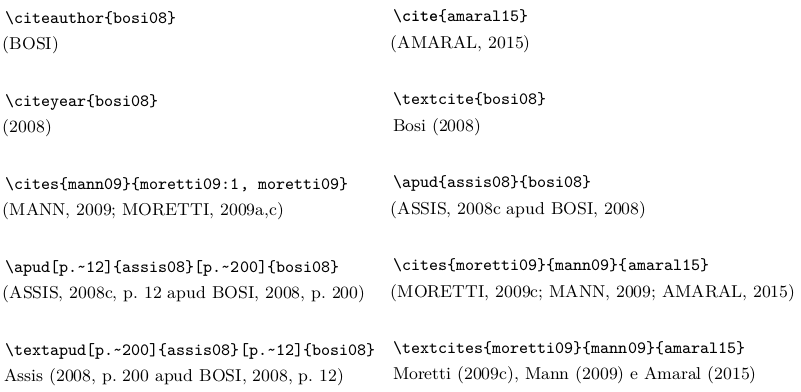
\includegraphics[width=0.8\textwidth,height=0.7\textheight,keepaspectratio]{figures/abnt-example.png}
\end{frame}


\begin{frame}[allowframebreaks,fragile]
\frametitle{Estilos de bibliografia}

\begin{lstlisting}[language=tex, label=lst-bibsty, caption={Escolhendo o estilo de bibliografia.}, postbreak=\mbox{$\hookrightarrow$\space}, basicstyle=\fontsize{8}{10}\selectfont\ttfamily]
\bibliographystyle{stylename}
\bibliography{bibfile}
\end{lstlisting}

\begin{figure}[h]
\centering
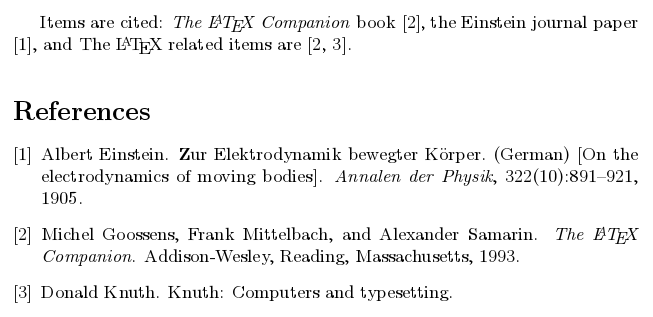
\includegraphics[width=0.8\textwidth,height=0.8\textheight,keepaspectratio]{figures/bib-plain.png}
\caption{Estilo \texttt{plain}.}
\label{fig-bib-plain}
\end{figure}

\framebreak

\begin{figure}[h]
\centering
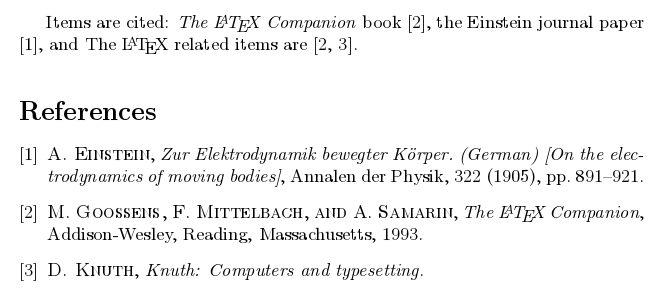
\includegraphics[width=0.8\textwidth,height=0.8\textheight,keepaspectratio]{figures/bib-siam.png}
\caption{Estilo \texttt{siam}.}
\label{fig-bib-siam}
\end{figure}

\framebreak

\begin{figure}[h]
\centering
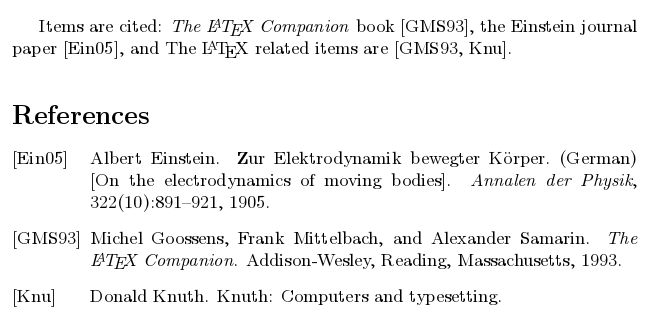
\includegraphics[width=0.8\textwidth,height=0.8\textheight,keepaspectratio]{figures/bib-alpha.png}
\caption{Estilo \texttt{alpha}.}
\label{fig-bib-alpha}
\end{figure}

\framebreak

\begin{itemize}
\item \hrefcolor{https://www.overleaf.com/learn/latex/Bibtex_bibliography_styles}{Overleaf - Bibtex bibliography styles}
\item \hrefcolor{http://www.mackichan.com/index.html?techtalk/632.htm~mainFrame}{MacKichan techtalk - BibTeX bibliography styles}
\item \hrefcolor{https://www.reed.edu/cis/help/LaTeX/bibtexstyles.html}{Reed College - Choosing a BibTeX Style}
\item \hrefcolor{http://www.cs.stir.ac.uk/~kjt/software/latex/showbst.html}{Ken Turner's - BibTeX Style Examples}
\end{itemize}

\end{frame}



\begin{frame}
\frametitle{Pacotes para formatação e programas para processar bibliografia}
Pacotes:
\begin{description}
\item[natbib] pacote antigo mas ainda muito utilizado 
\item[biblatex] pacote em desenvolvimento ativo conjuntamente com o \texttt{biber}
\end{description}

Programas:
\begin{description}
\item[bibtex] estável e amplamente utilizado
\item[biber] capaz de lidar com mais tipos de entrada e campos, suporte à codificação UTF-8, maior controle no ordenamento (funciona apenas com \texttt{biblatex})
\end{description}

Mais informações: \url{https://tex.stackexchange.com/questions/25701/bibtex-vs-biber-and-biblatex-vs-natbib}.
\end{frame}


\begin{frame}
\frametitle{Dica - Bibliografia}

\begin{itemize}
 \item \hrefcolor{https://zbib.org/}{zoterobib}
 \item \hrefcolor{https://www.doi2bib.org/}{https://www.doi2bib.org/}
 \item \hrefcolor{https://books.google.com}{Google Books}
 \item \hrefcolor{https://www.xarg.org/tools/isbn-to-bibtex/}{https://www.xarg.org/tools/isbn-to-bibtex/}
 \item \hrefcolor{https://www.ottobib.com/}{https://www.ottobib.com/} 
 \item \hrefcolor{https://manas.tungare.name/software/isbn-to-bibtex}{https://manas.tungare.name/software/isbn-to-bibtex}
 \item \hrefcolor{https://arxiv2bibtex.org/}{https://arxiv2bibtex.org/}
\end{itemize}

\vspace{3ex}
Existem ainda vários pacotes para fazer citações, epígrafes, etc.
Veja alguns exemplos no \hrefcolor{https://www.overleaf.com/learn/latex/Typesetting_quotations}{Overleaf}.

\end{frame}



\begin{frame}[fragile,allowframebreaks]
\frametitle{Acrônimos}

Pacote \texttt{acronym} disponível em: \url{https://www.ctan.org/pkg/acronym}.

\begin{verbatim}
\usepackage{acronym}
\end{verbatim}



Opções:
\begin{description}
\item[footnote] nome completo aparece como nota de rodapé
\item[nohyperlinks] não faz o link com glossário 
\item[printonlyused] imprime apenas os que forem utilizados
\item[withpage] imprime a página onde foram utilizados pela primeira vez
\item[smaller] utiliza uma fonte menor
\item[nolist] não faz a lista de acrônimos
\end{description}


\begin{LTXexample}
\begin{acronym}
\acro{CTAN}{The Comprehensive \TeX{} Archive Network}
\acro{RMS}{Root-Mean-Square}
\end{acronym}

\lipsum[1][1-2] \ac{CTAN} \lipsum[1][3] \ac{RMS}.
\lipsum[1][4] \ac{CTAN}, \lipsum[1][5] \ac{RMS}.
\end{LTXexample}

\end{frame}
